\documentclass[]{article}
\usepackage[utf8]{inputenc}
\usepackage{natbib}
\usepackage{amsmath}
\usepackage{amssymb}
\usepackage{relsize}
\usepackage{graphicx}

\title{\textbf{CSDS 391: W4}}
\author{John Mays, \texttt{jkm100}}
\date{Due 11/02/21, Professor Lewicki}

\begin{document}

\maketitle

\newcommand{\st}{\text{ s.t. }}
\newcommand{\false}{\textbf{F}}

\section*{Q1}
\subsection*{a)}
Normalizing constant:
$$p(y|n)=\int^{1}_0 p(y|\Theta, n)p(\Theta,n)d\Theta=\int^{1}_0 p(y|\Theta, n)d\Theta=\frac{1}{1+n}$$
Posterior:
$$p(\Theta|y,n)=\frac{p(y|\Theta, n)p(\Theta|n)}{p(y|n)}=p(y|\Theta, n)p(\Theta|n)(1+n)$$
\subsection*{b)}
\begin{center}
    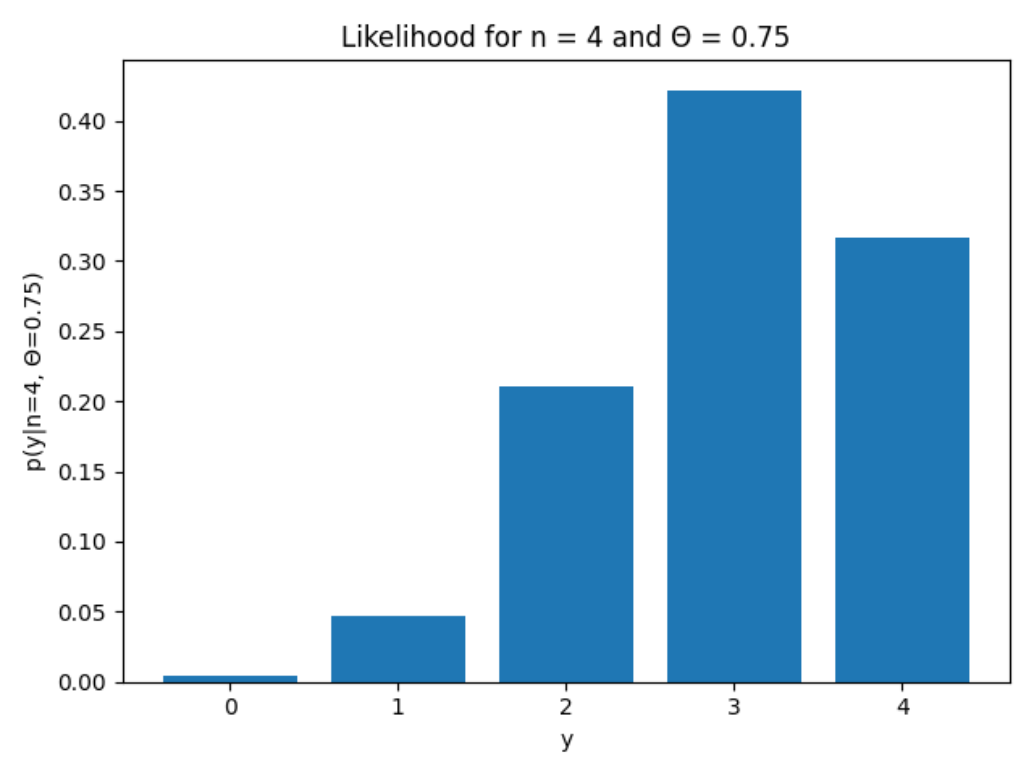
\includegraphics[scale = 0.5]{1_b.png}
\end{center}
\pagebreak
\subsection*{c)} 
\begin{center}
    \begin{tabular}{cc}
        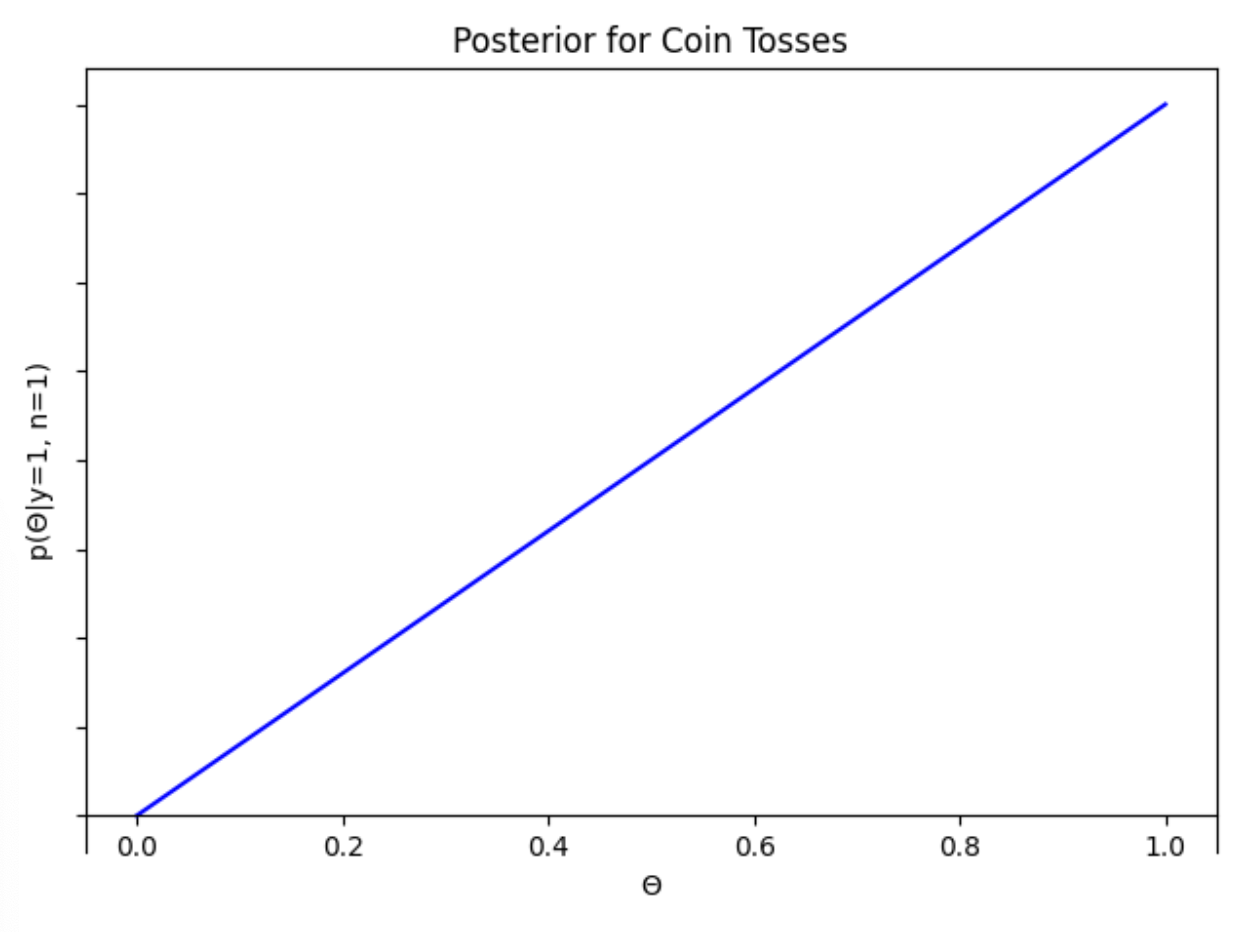
\includegraphics[scale = 0.25]{1_c_1.png} & 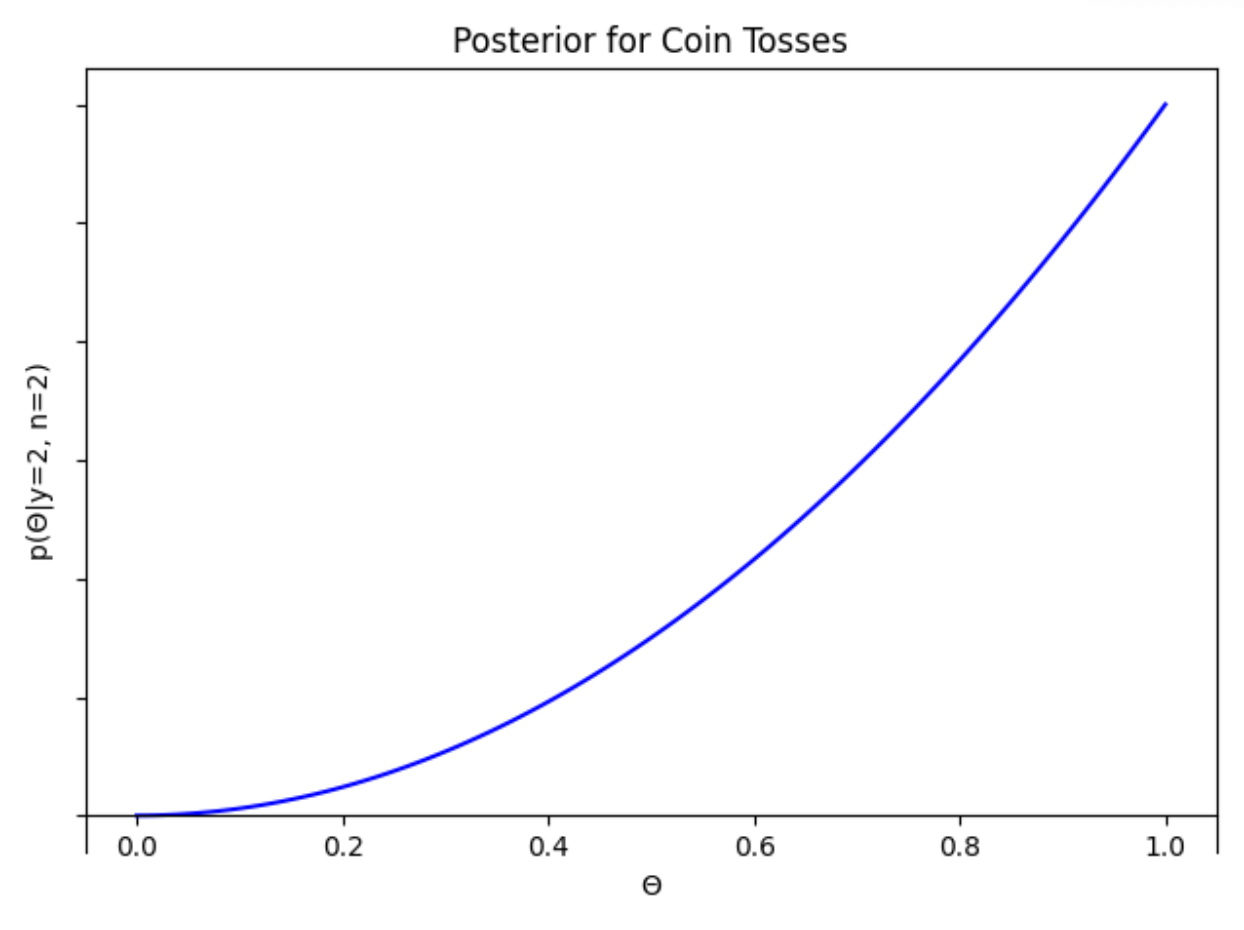
\includegraphics[scale = 0.25]{1_c_2.png}\\
        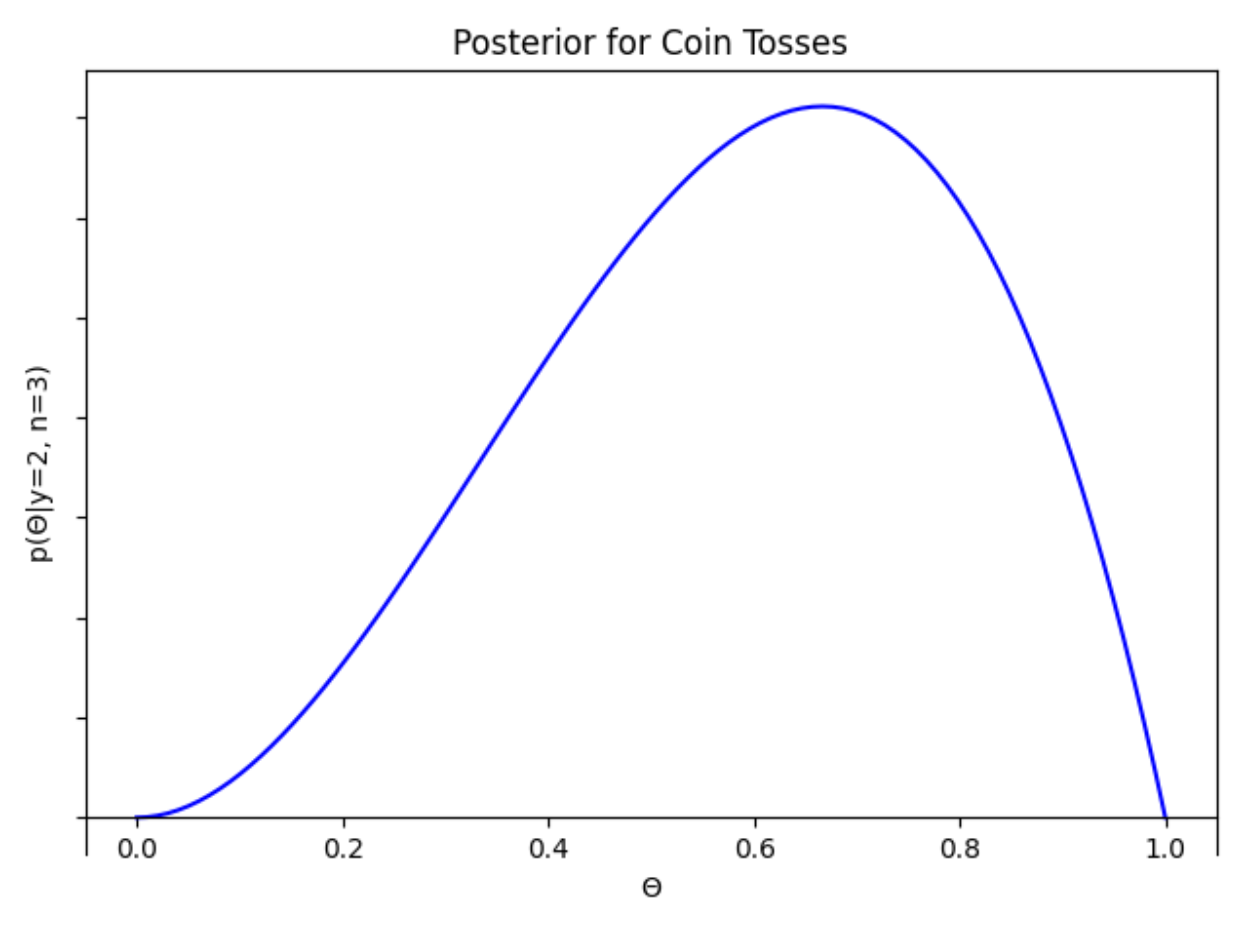
\includegraphics[scale = 0.25]{1_c_3.png} & 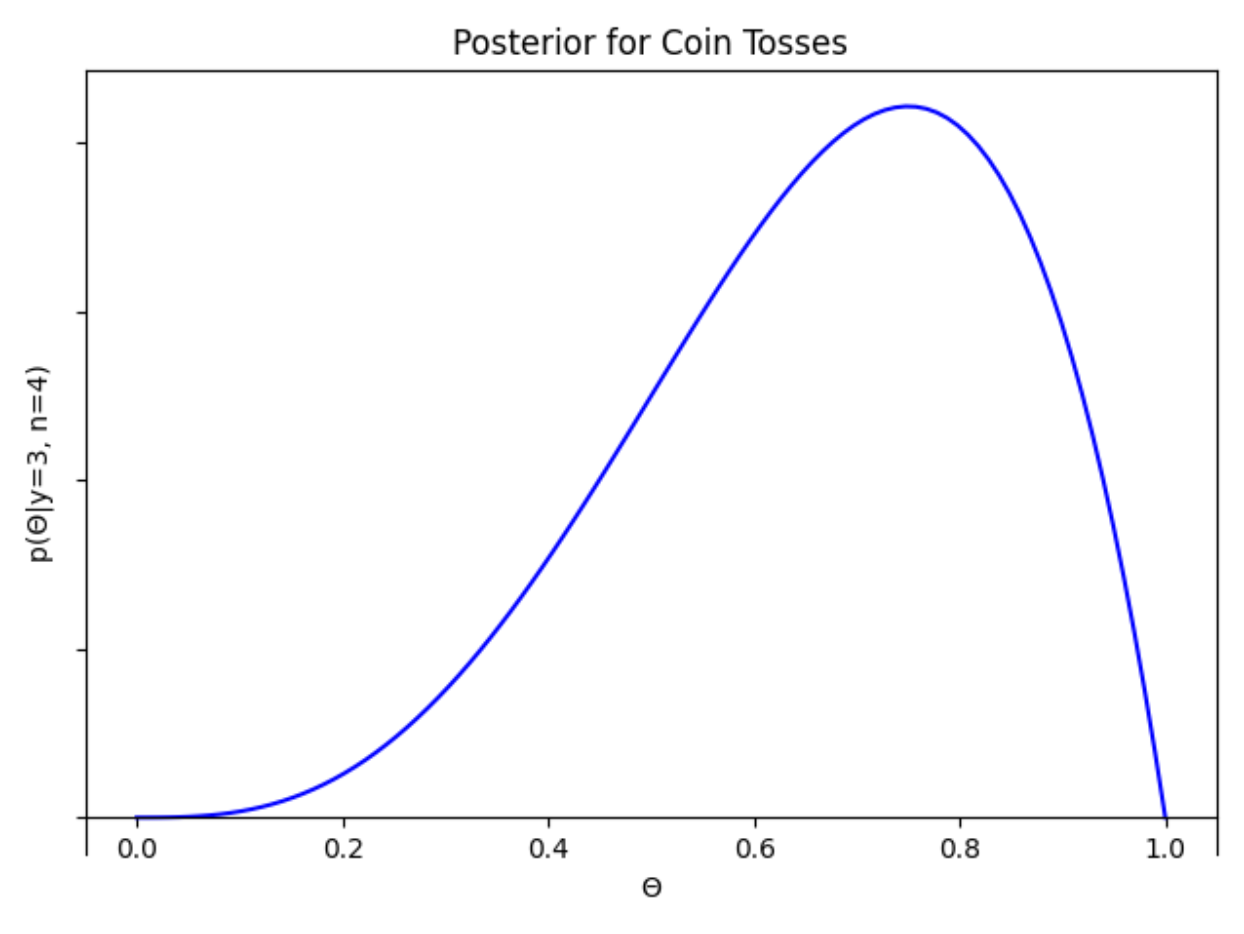
\includegraphics[scale = 0.25]{1_c_4.png}
    \end{tabular}
\end{center}
\pagebreak
\section*{Q2}
\subsection*{a)}
\textbf{h1:}
\begin{center}
    \begin{tabular}{cc}
    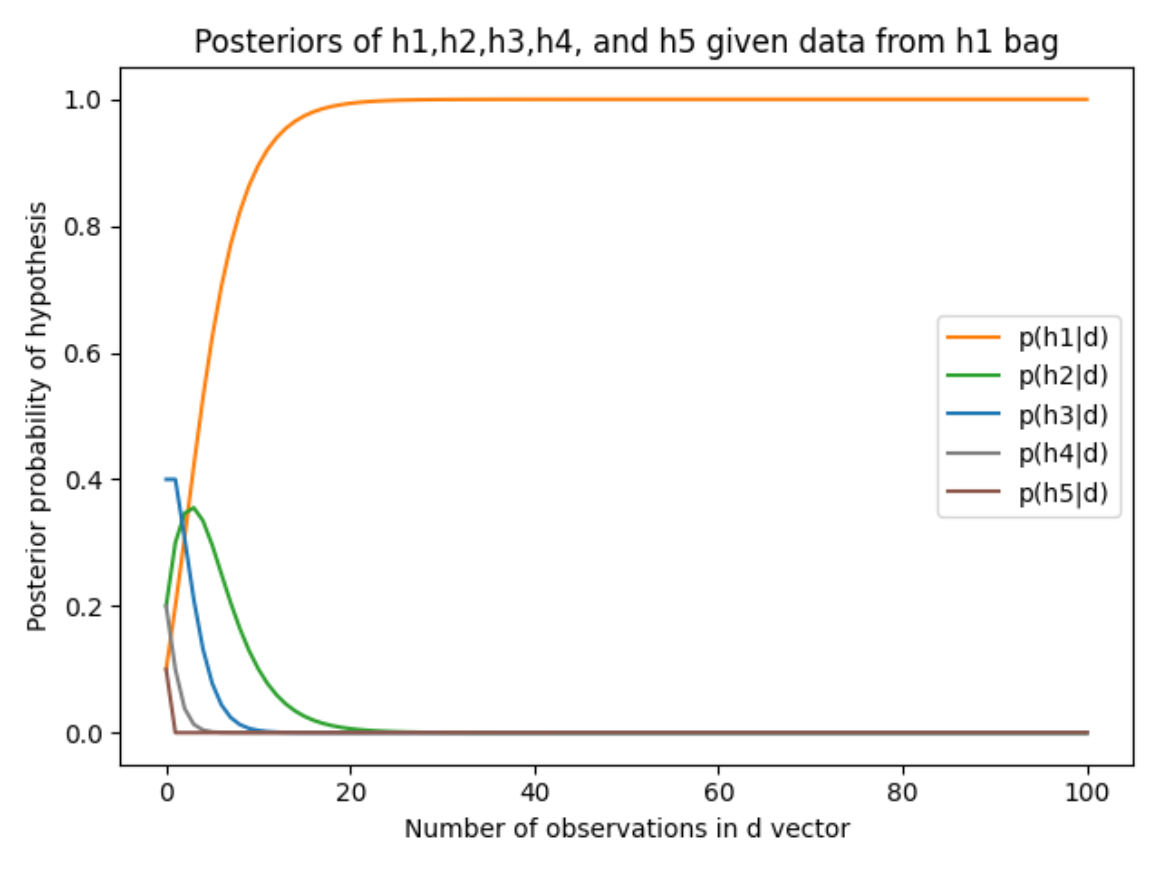
\includegraphics[scale = 0.30]{2_a_posteriors_h1.png} & 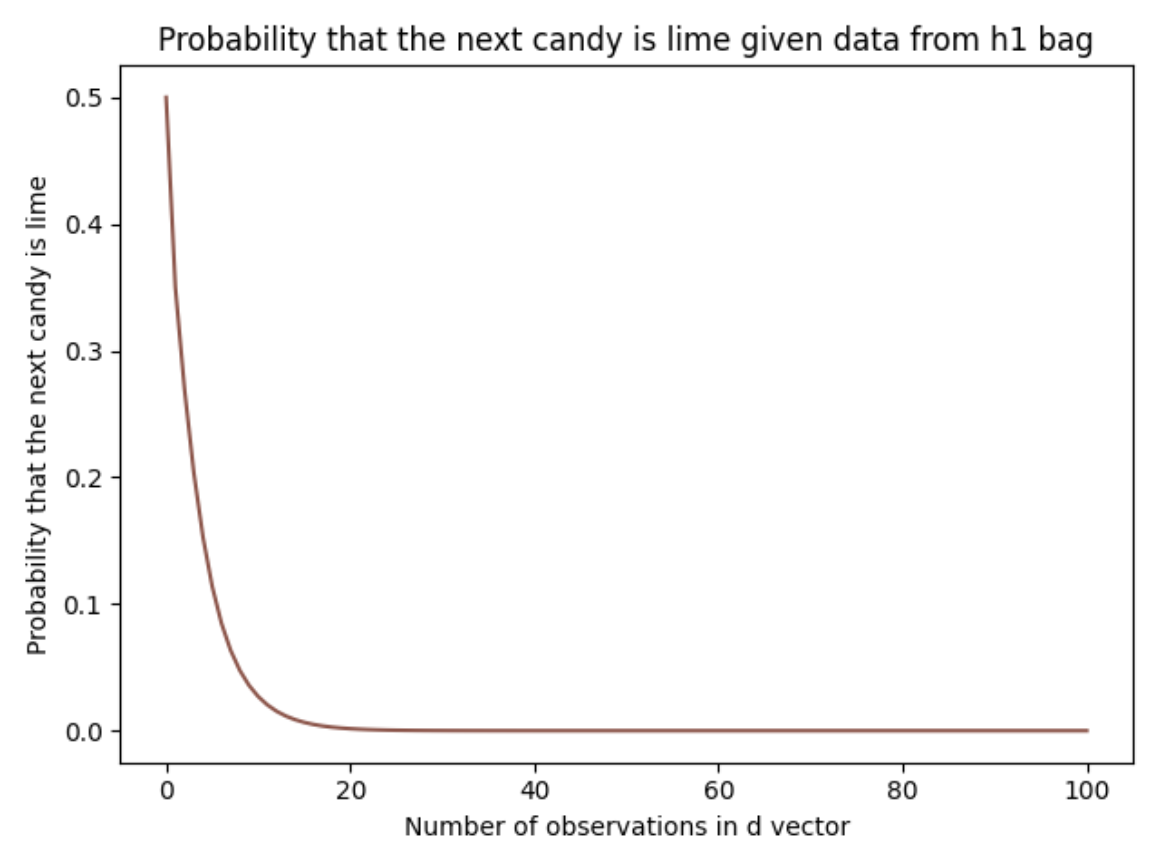
\includegraphics[scale = 0.30]{2_a_lime_h1.png} 
\end{tabular}
\end{center}
\textbf{h2:}
\begin{center}
    \begin{tabular}{cc}
    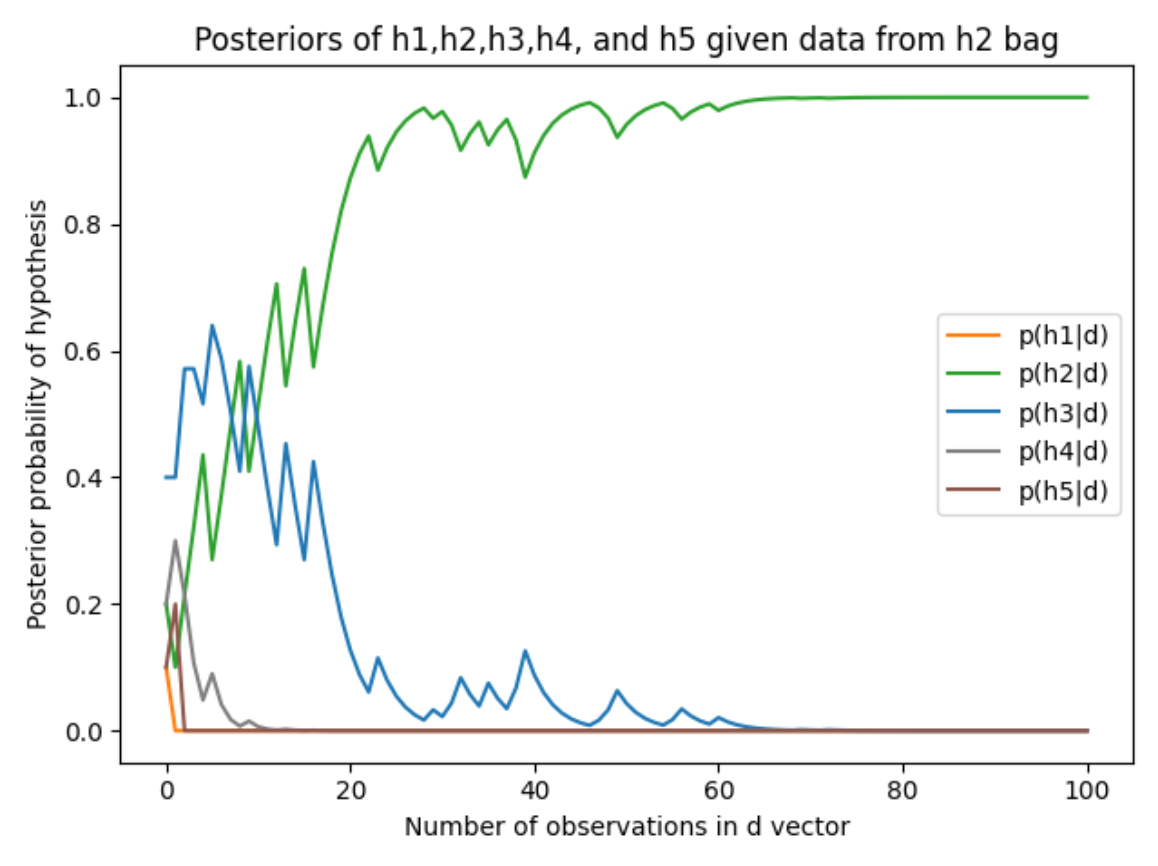
\includegraphics[scale = 0.30]{2_a_posteriors_h2.png} & 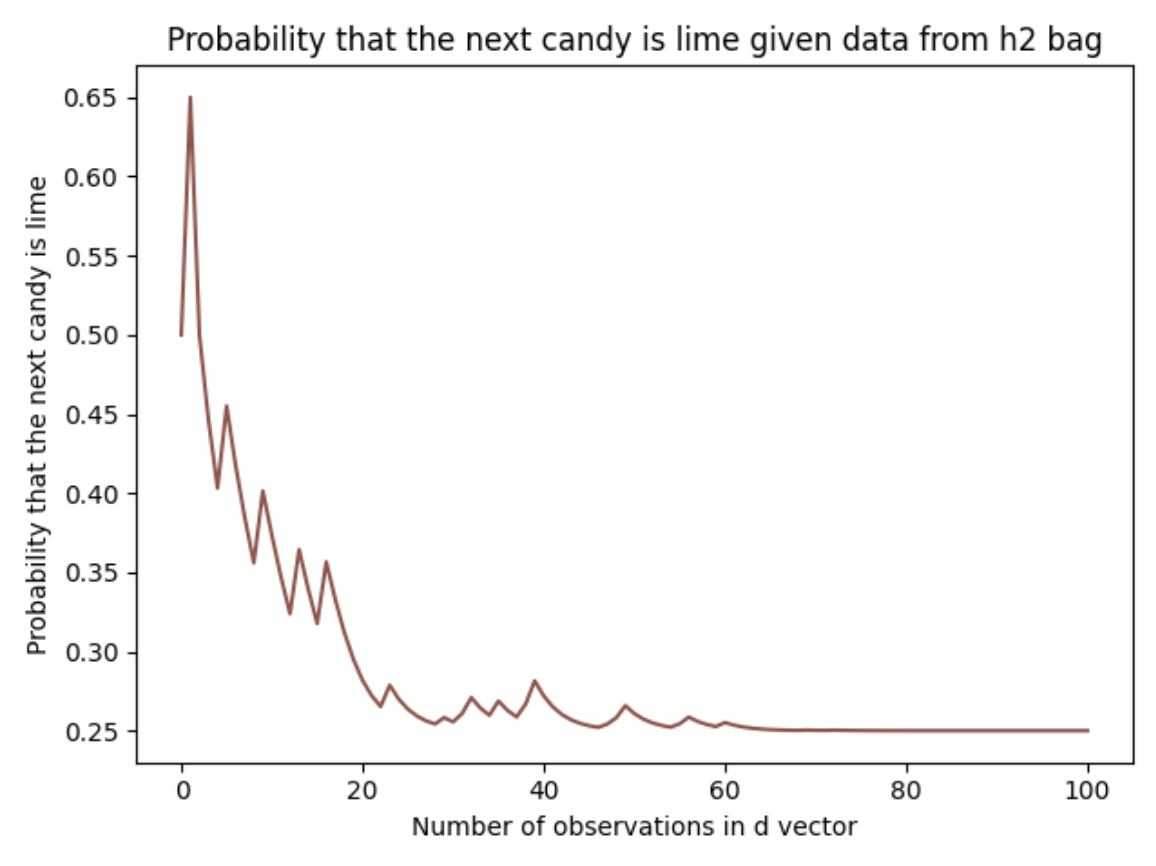
\includegraphics[scale = 0.30]{2_a_lime_h2.png} 
\end{tabular}
\end{center}
\textbf{h3:}
\begin{center}
    \begin{tabular}{cc}
    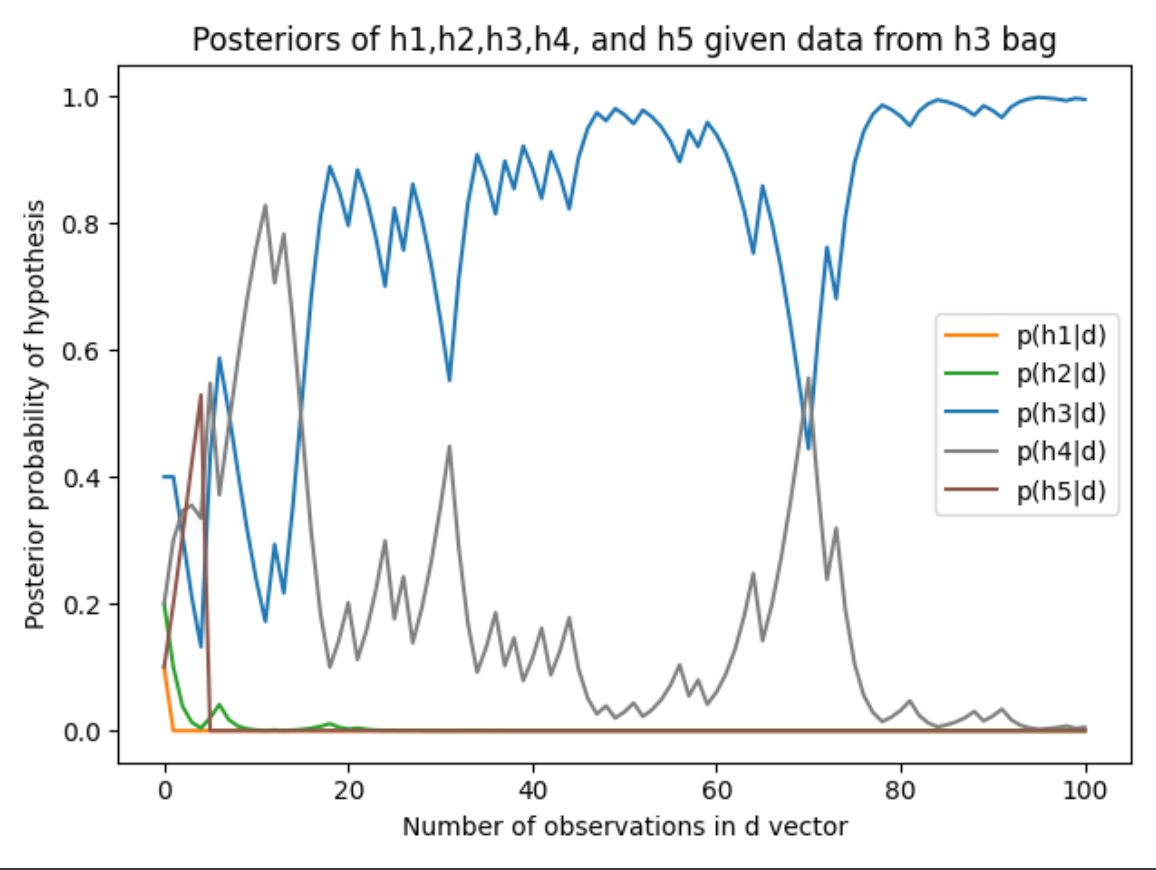
\includegraphics[scale = 0.30]{2_a_posteriors_h3.png} & 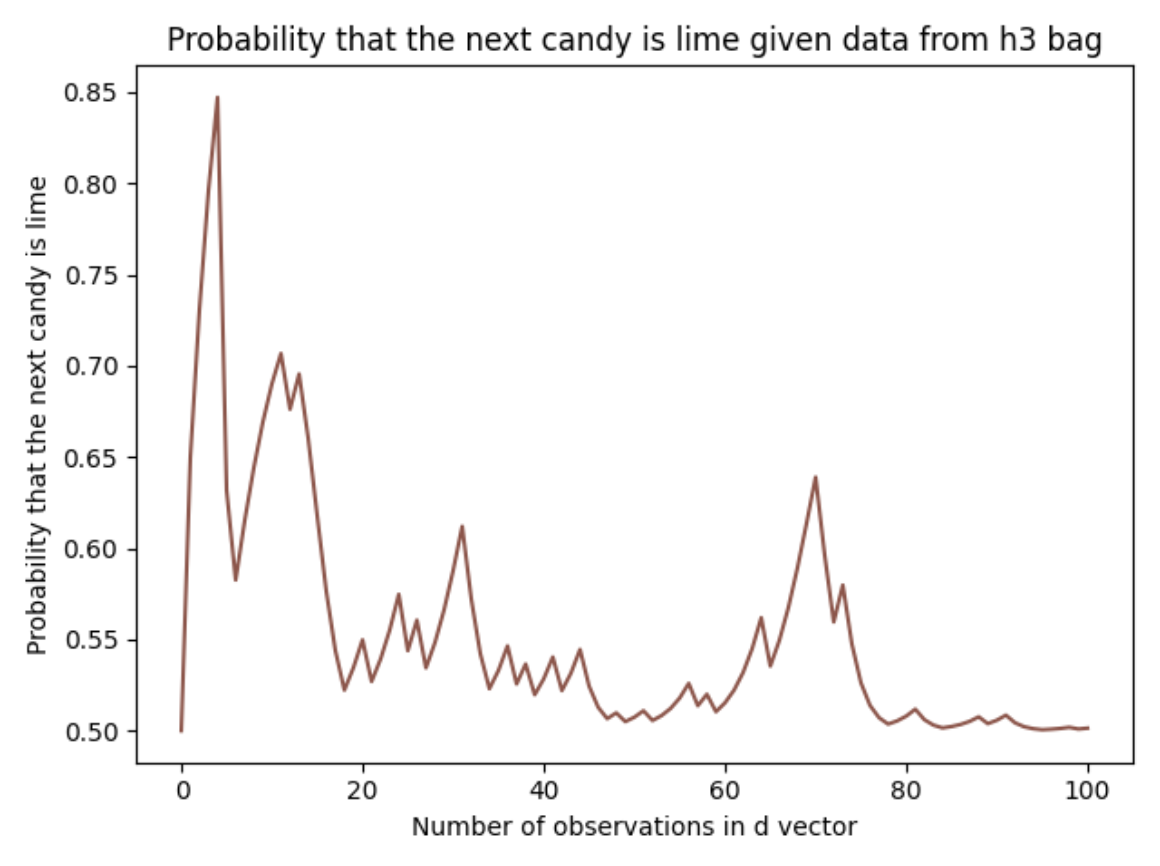
\includegraphics[scale = 0.30]{2_a_lime_h3.png} 
\end{tabular}
\end{center}
\textbf{h4:}
\begin{center}
    \begin{tabular}{cc}
    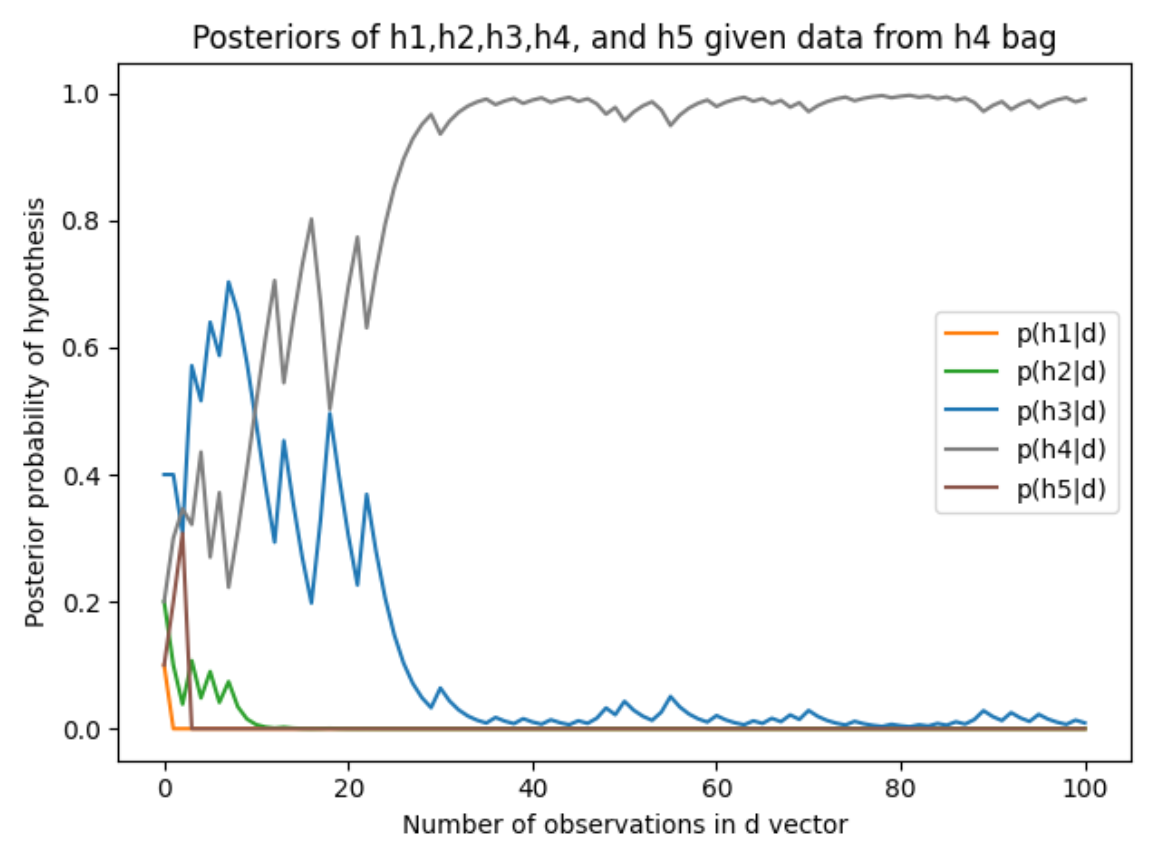
\includegraphics[scale = 0.30]{2_a_posteriors_h4.png} & 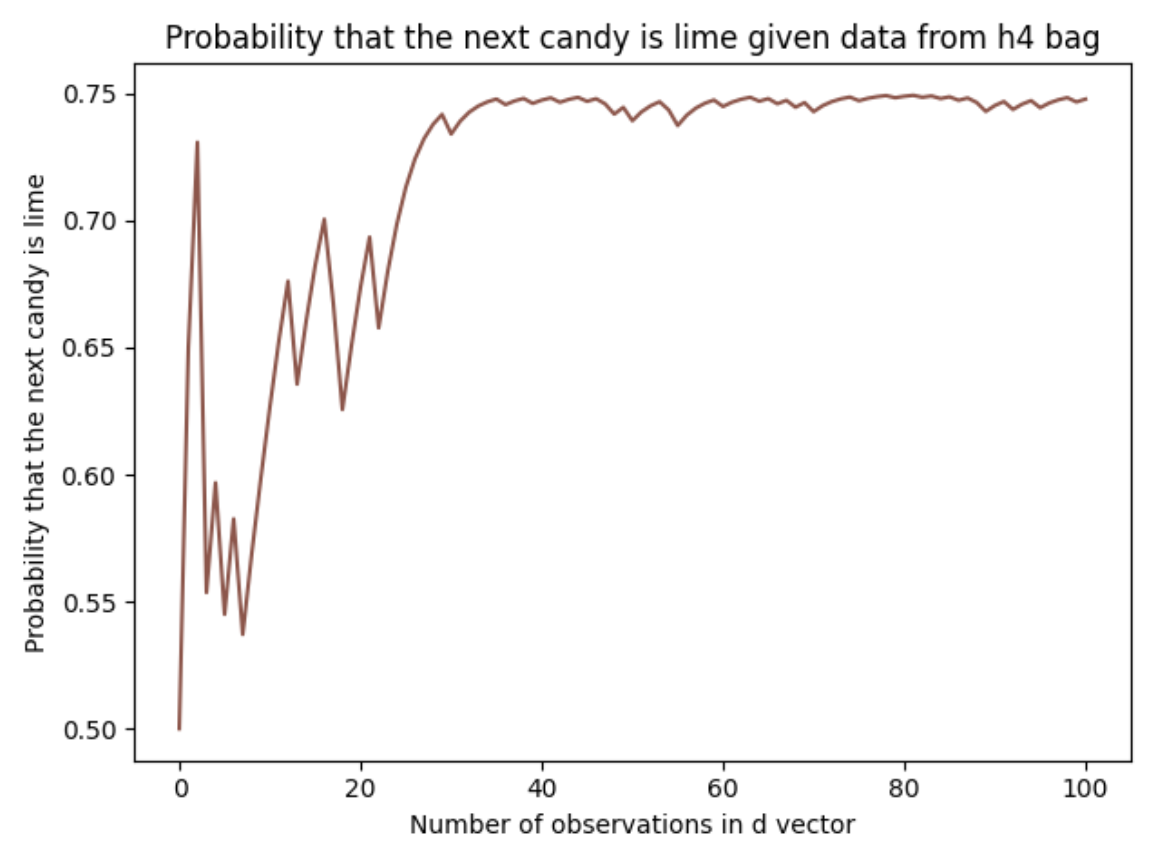
\includegraphics[scale = 0.30]{2_a_lime_h4.png} 
\end{tabular}
\end{center}
\subsection*{b)}
Given a data vector $\textbf{d}$ with $N$ data points, and understanding that $\textbf{d}_i$ is the data vector of length $i$ with the first $i$ observations from $\textbf{d}$, $0\leq i \leq N$, then
$$\min(i), \st i\text{ satisfies }\max(\begin{bmatrix} P(h_1|\textbf{d}_i)\\ P(h_2|\textbf{d}_i)\\ P(h_3|\textbf{d}_i)\\ P(h_4|\textbf{d}_i)\\ P(h_5|\textbf{d}_i)\\\end{bmatrix})> 0.9$$
will return the minimum value of $i$ for which any hypothesis, given $\textbf{d}_i$, will return a probability of $>$ $90\%$.  Then, $i$ is the number of observations you have to make until you can be more than $90\%$ sure of which bag you have.\\  
\linebreak
For example, say you generated data vector $\textbf{d}$ from a bag of candies satisfying one hypothesis.  You would consider the set of values of $i$ from $0$ to $N$ that satisfy the inequality.  The inequality considers the most probable hypothesis, given data vector $\textbf{d}_i$, and sees if it is greater than $0.9$. The function returns the minimum value of $i$ that satisfies the inequality, otherwise stated as the number of the first observation that leads to a posterior probability of greater than $90\%$.
\subsection*{c)}
For this question, I did essentially the same exact steps as part \textbf{2a}, only each data point is an average of $2500$ runs of \textbf{2a}.
\begin{gather*}
    \begin{tabular}{cc}
    Bag satisfying \textbf{h1}: & Bag satisfying \textbf{h2}:\\
    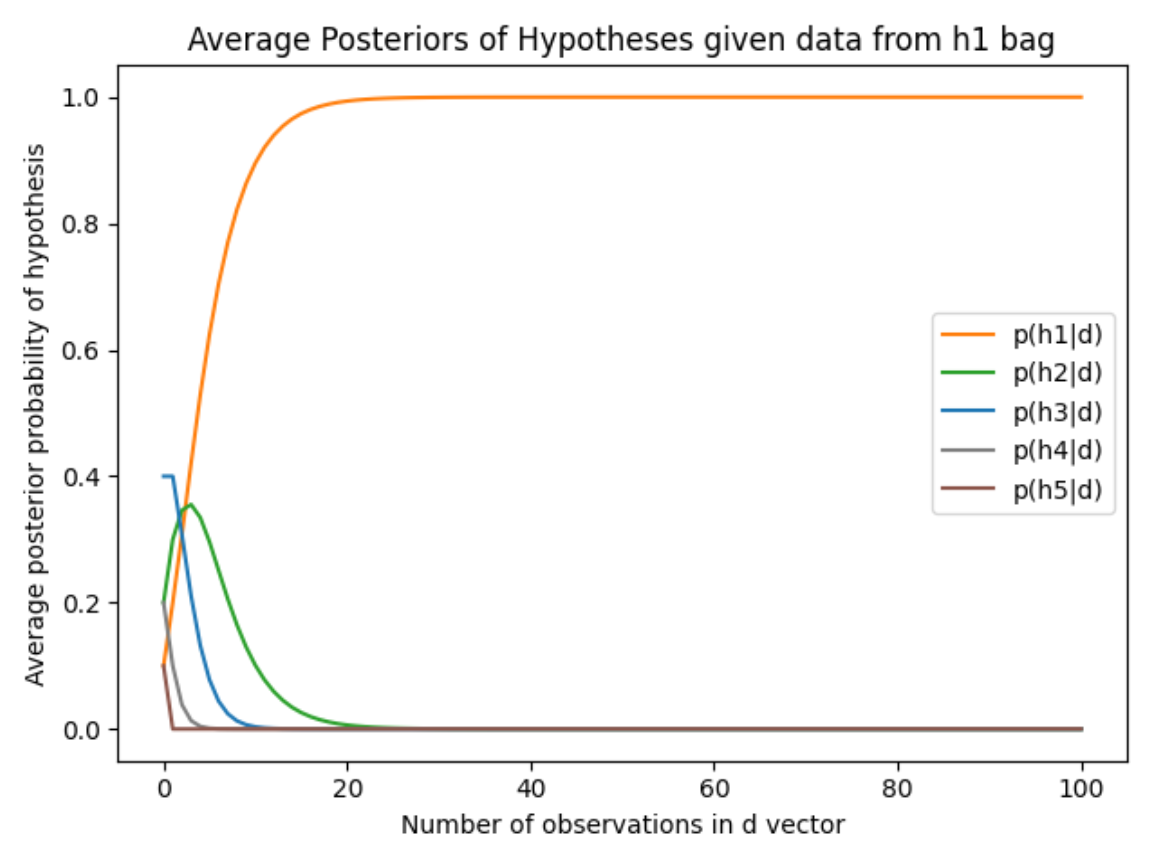
\includegraphics[scale=0.3]{2_c_h1.png} & 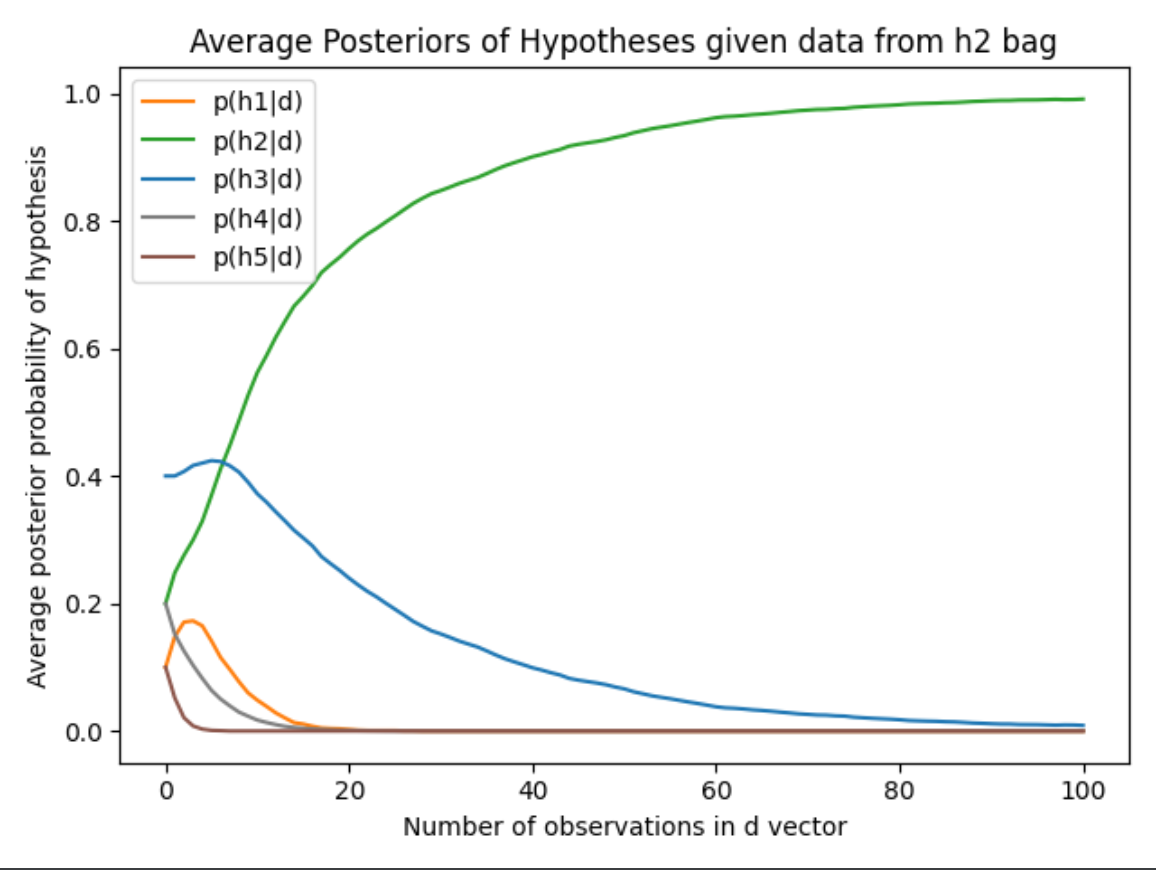
\includegraphics[scale=0.3]{2_c_h2.png}
    \end{tabular}\\
    \begin{tabular}{cc}
    Bag satisfying \textbf{h3}: & Bag satisfying \textbf{h4}:\\
    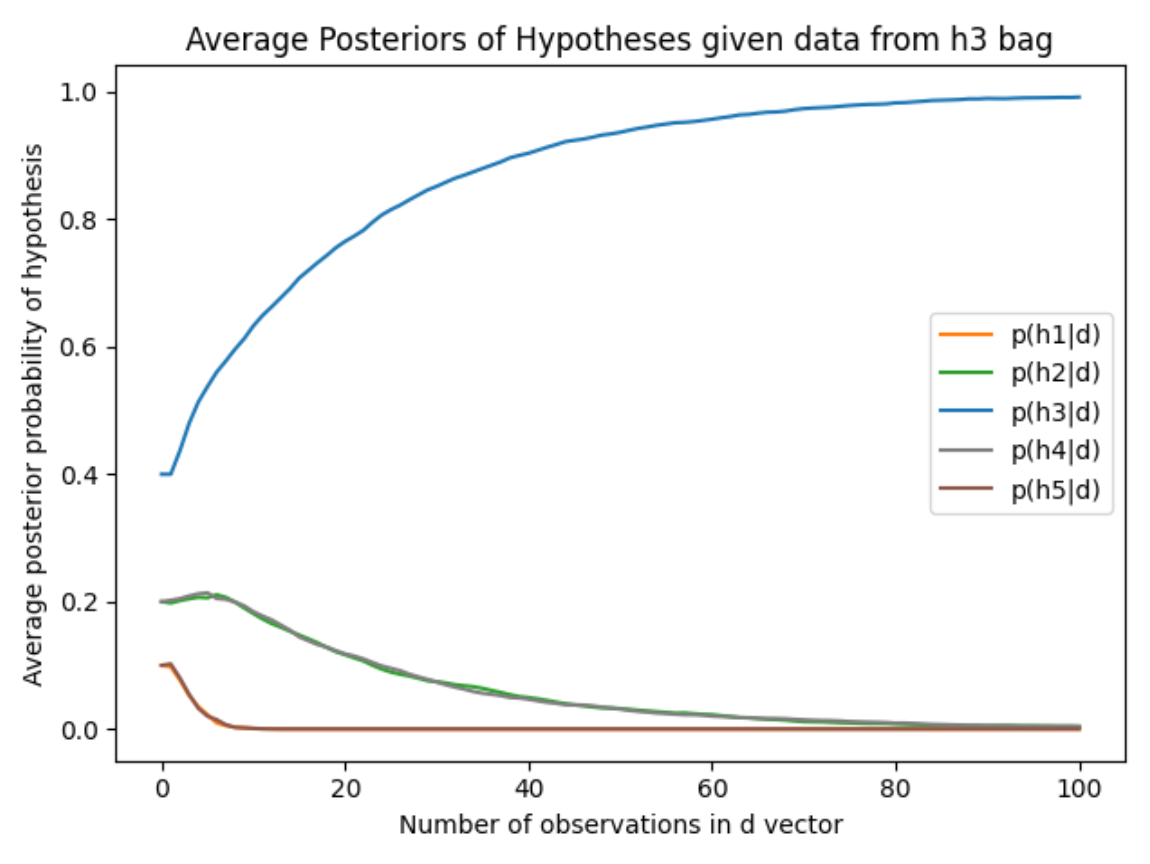
\includegraphics[scale=0.3]{2_c_h3.png} & 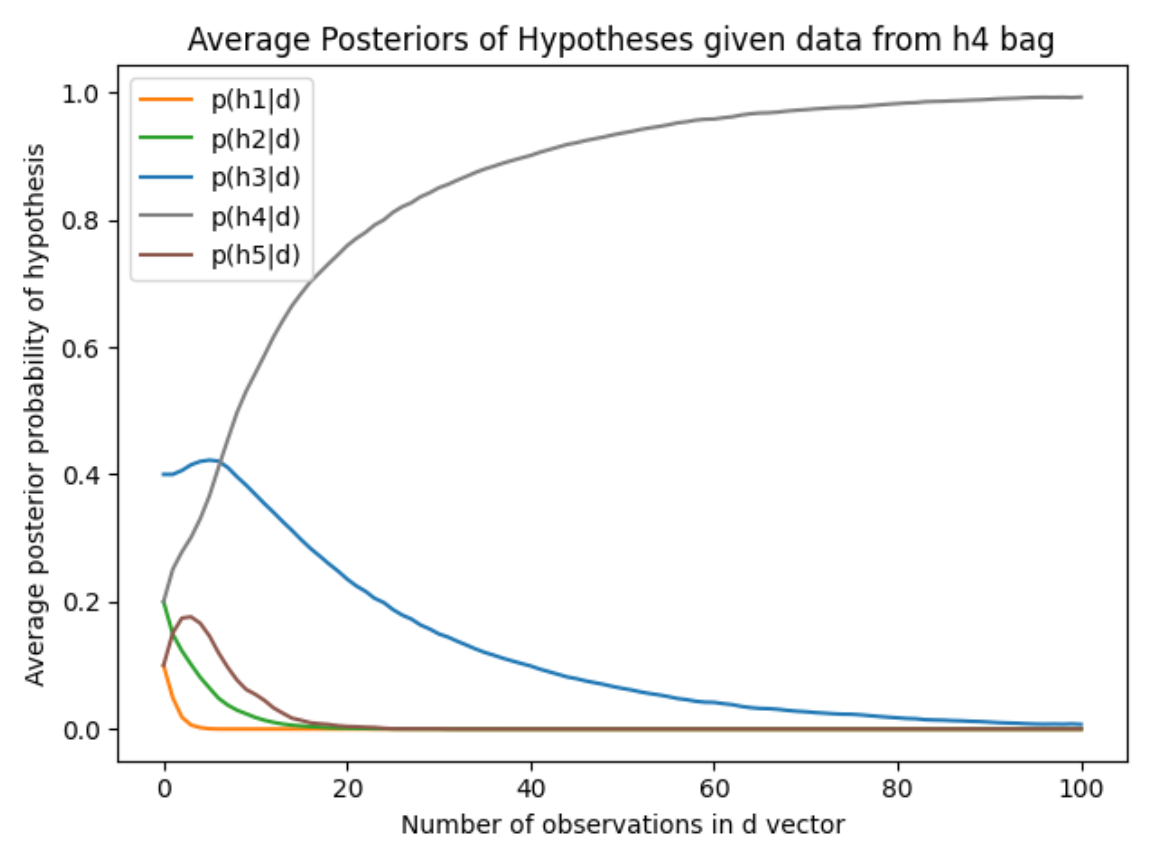
\includegraphics[scale=0.3]{2_c_h4.png}
    \end{tabular}\\
    \begin{tabular}{c}
    Bag satisfying \textbf{h5}:\\
    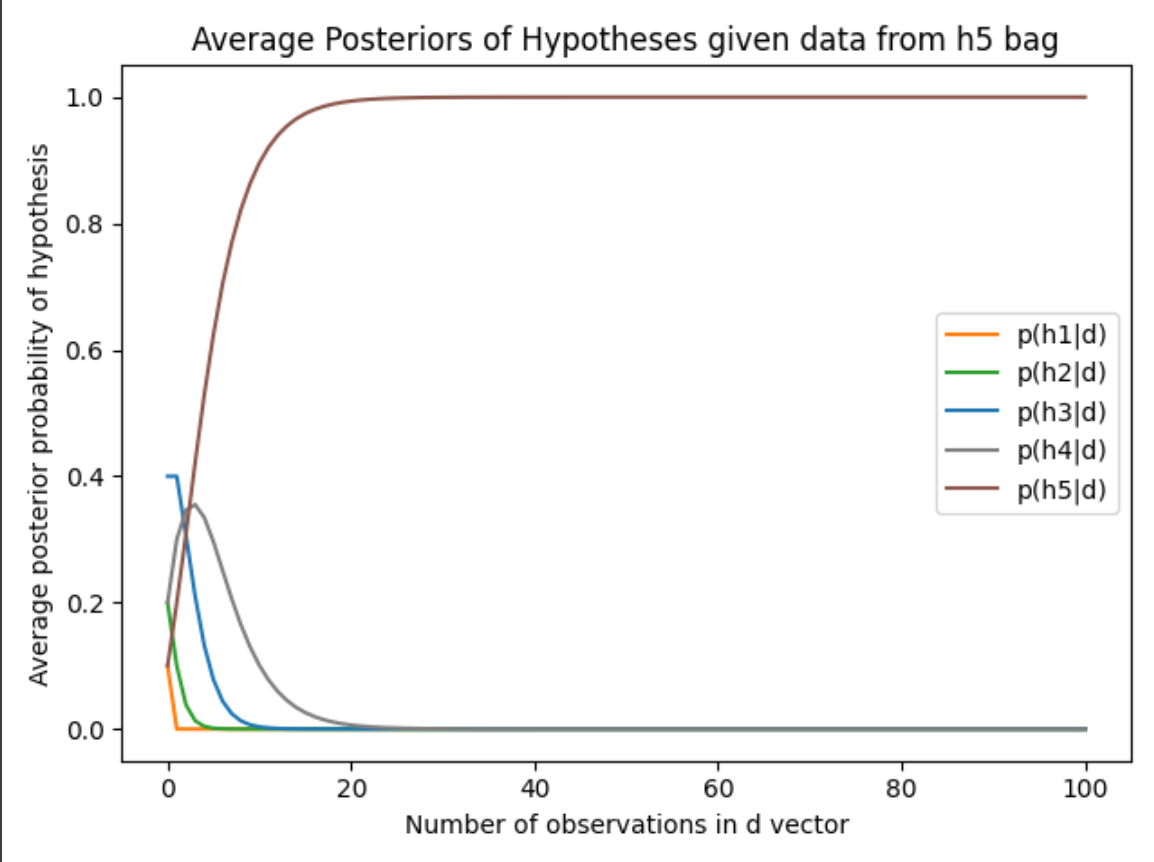
\includegraphics[scale=0.3]{2_c_h5.png}
    \end{tabular}
\end{gather*}
\section*{Q3}
The objective function, distortion, is given as
\begin{gather*}
    D = \sum^{N}_{n=1} \sum^{K}_{k=1} r_{n,k} || \textbf{x}_{n} - \boldsymbol\mu_{k} ||^{2}
\end{gather*}
The update rule is supposed to minimize this function, therefore we can take the gradient and set it equal to zero:
\begin{gather*}
    \frac{\partial D}{\partial \boldsymbol\mu_{k}}=2\sum^{N}_{n=1}r_{n,k}(\textbf{x}_{n} - \boldsymbol\mu_{k})\\
    = 2\sum^{N}_{n=1}r_{n,k}\textbf{x}_{n} - 2\sum^{N}_{n=1}r_{n,k}\boldsymbol\mu_{k} = 0 \implies\\
    \sum^{N}_{n=1}r_{n,k}\boldsymbol\mu_{k} = \sum^{N}_{n=1}r_{n,k}\textbf{x}_{n}
\end{gather*}
Since the $\boldsymbol\mu_{k}$ vector is the same across the entire sum on the left side, we can take it out as a constant:
\begin{gather*}
    \boldsymbol\mu_{k} \sum^{N}_{n=1}r_{n,k} = \sum^{N}_{n=1}r_{n,k}\textbf{x}_{n} \implies \\
    \boldsymbol\mu_{k} = \frac{\mathlarger{\sum^{N}_{n=1}}r_{n,k}\textbf{x}_{n}}{\mathlarger{\sum^{N}_{n=1}}r_{n,k}}
\end{gather*}
In other words, the gradient with respect to $\boldsymbol\mu_{k}$ is equal to $0$ when $\boldsymbol\mu_{k}$ is equal to the average value of the data vectors $\textbf{x}_{n}$ belonging to class $k$.\\
The same can be said for the individual values of $\boldsymbol\mu_{k}$, $\mu_{k,i}$:
\begin{gather*}
    \mu_{k,i} = \frac{\mathlarger{\sum^{N}_{n=1}}r_{n,k}x_{n,i}}{\mathlarger{\sum^{N}_{n=1}}r_{n,k}}
\end{gather*}
\linebreak
Given these two equations, we can formulate our update rule as:
\begin{itemize}
    \item update mean $\boldsymbol\mu_{k}$ to satisfy equations (listed below)
    \item repeat until convergence
\end{itemize}
\begin{gather*}
    \textbf{scalar form equation:}\\
    \mu_{k,i} = \frac{\mathlarger{\sum^{N}_{n=1}}r_{n,k}x_{n,i}}{\mathlarger{\sum^{N}_{n=1}}r_{n,k}}\\
    \textbf{vector form equation:}\\
    \boldsymbol\mu_{k} = \frac{\mathlarger{\sum^{N}_{n=1}}r_{n,k}\textbf{x}_{n}}{\mathlarger{\sum^{N}_{n=1}}r_{n,k}}
\end{gather*}


\end{document}